
\documentclass[12pt]{article}
\usepackage[utf8]{inputenc}
\usepackage[utf8]{vietnam}
\AtBeginDocument{%
  \renewcommand{\contentsname}{Contents}
  \renewcommand{\listfigurename}{List of Figures}
  \renewcommand{\listtablename}{List of Tables}
  \renewcommand{\refname}{References}
  \renewcommand{\indexname}{Index}
  \renewcommand{\figurename}{Figure}
  \renewcommand{\tablename}{Table}
  \renewcommand{\partname}{Part}
  \renewcommand{\appendixname}{Appendix}
}
\usepackage{graphicx}
\usepackage{geometry}
\geometry{a4paper, margin=2cm}
\usepackage{amsmath}
\usepackage{amssymb}
\usepackage{booktabs}
\usepackage{listings}
\usepackage{xcolor}
\usepackage{caption}
\usepackage{float}
\usepackage[hyphens]{url}
\usepackage{ragged2e}
\usepackage[bookmarks=true, bookmarksopen=true, bookmarksnumbered=true, colorlinks=true, linkcolor=black, urlcolor=blue, citecolor=black]{hyperref}

\definecolor{codegreen}{rgb}{0,0.6,0}
\definecolor{codegray}{rgb}{0.5,0.5,0.5}
\definecolor{codepurple}{rgb}{0.58,0,0.82}
\definecolor{backcolour}{rgb}{0.95,0.95,0.92}

\lstdefinestyle{mystyle}{
    backgroundcolor=\color{backcolour},   
    commentstyle=\color{codegreen},
    keywordstyle=\color{magenta},
    numberstyle=\tiny\color{codegray},
    stringstyle=\color{codepurple},
    basicstyle=\ttfamily\footnotesize,
    breakatwhitespace=false,         
    breaklines=true,                 
    captionpos=b,                    
    keepspaces=true,                 
    numbers=left,                    
    numbersep=5pt,                  
    showspaces=false,                
    showstringspaces=false,
    showtabs=false,                  
    tabsize=2
}

\lstset{style=mystyle}
\graphicspath{ {./results/} }

\begin{document}

\begin{titlepage}
    \centering
    {\large \textbf{UNIVERSITY OF SCIENCE AND TECHNOLOGY OF HANOI} \par}
    \vspace{4cm}
    
\includegraphics[width=0.6\textwidth]{../lab3/usth.png} \par
    \vspace{3cm}
    {\Large \textbf{MACHINE LEARNING AND DATA MINING II} \par}
    \vspace{0.5cm}
    {\Large \textbf{LABWORK 4: CLASSIFICATION II} \par}
    \vfill
    {\large \textbf{TẠ HIẾU NAM (22BI13327)} \par}
    \vspace{0.3cm}
    {\large \textbf{ĐỖ DUY TOÀN (22BI13420)} \par}
    \vspace{2cm}
    \vfill
    {\large \textbf{Lecturer: Dr. Đoàn Nhật Quang} \par}
    \vspace{1.5cm}
    \thispagestyle{empty}
\end{titlepage}

\pagenumbering{roman}
\tableofcontents
\newpage
\listoftables
\listoffigures
\newpage

\pagenumbering{arabic}
\justifying

\section{Decision Tree - DT}

The objective of this section is to investigate the performance of the Decision Tree algorithm, a fundamental non-parametric supervised learning method, on high-dimensional classification tasks.

\subsection{Select two datasets with labels available}

To evaluate the versatility of the decision tree model, we selected two distinct datasets representing different domains and feature types:

\begin{enumerate}
    \item \textbf{Mice Protein Expression:} A biological dataset comprising 1080 samples from control, trisomic, and drug-treated mice. Each sample is characterized by 77 continuous features representing protein expression levels. The target variable consists of 8 distinct classes based on genotype, behavior, and treatment.
    \item \textbf{ISOLET (Isolated Letter Speech Recognition):} A speech processing dataset containing 7797 samples of spoken English alphabet letters (26 classes). Each sample is described by 617 continuous features derived from spectral analysis of the audio signal.
\end{enumerate}

\subsection{Analyze and pre-process the data}

\subsubsection{Data Analysis}
Before applying any learning algorithm, it is critical to understand the underlying structure of the data. 

\paragraph{Class Distribution.} We analyzed the distribution of samples across classes to check for imbalance.
\begin{itemize}
    \item For \textbf{Mice Protein} (Figure \ref{fig:mice_dist}), the classes are distributed relatively evenly, ensuring that the model will not be biased towards any majority class.
    \item For \textbf{ISOLET} (Figure \ref{fig:isolet_dist}), the distribution is perfectly uniform, which is ideal for multi-class classification training.
\end{itemize}

\begin{figure}[H]
    \centering
    \begin{minipage}{0.48\textwidth}
        \centering
        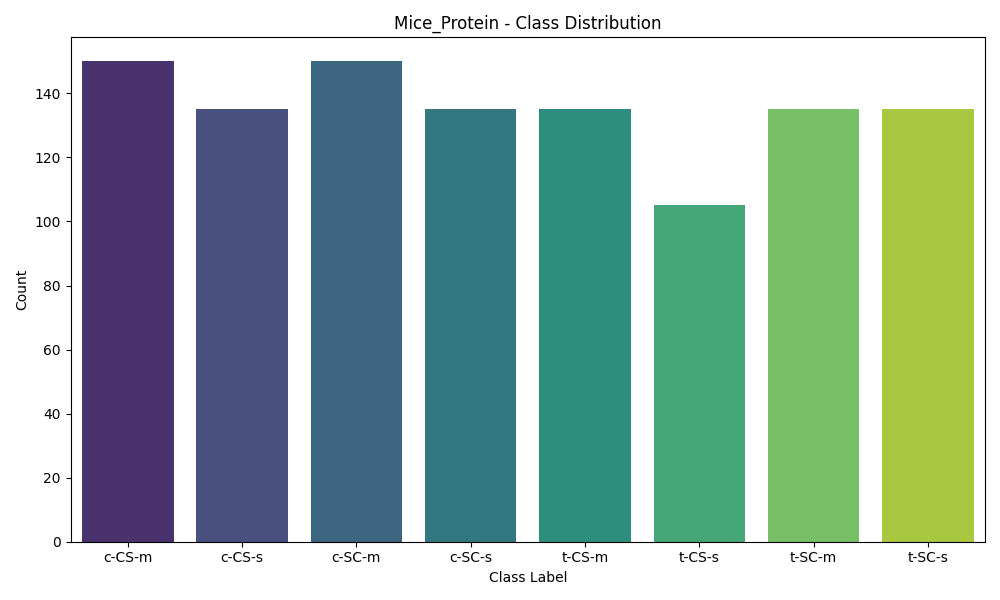
\includegraphics[width=\linewidth]{Mice_Protein_dist.png}
        \caption{Class Distribution (Mice Protein)}
        \label{fig:mice_dist}
    \end{minipage}
    \hfill
    \begin{minipage}{0.48\textwidth}
        \centering
        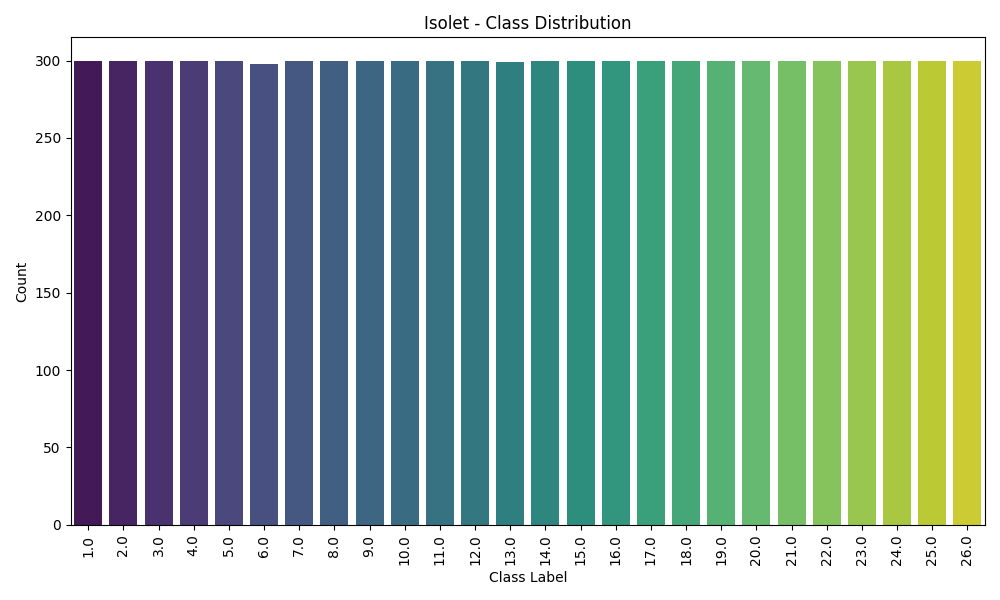
\includegraphics[width=\linewidth]{Isolet_dist.png}
        \caption{Class Distribution (Isolet)}
        \label{fig:isolet_dist}
    \end{minipage}
\end{figure}

\paragraph{Dimensionality and Separability (PCA).} Given the high dimensionality of the datasets (77 and 617 features), we employed Principal Component Analysis (PCA) to project the data into a 2D space for visualization. Figures \ref{fig:mice_pca} and \ref{fig:isolet_pca} show the first two principal components. 
\begin{itemize}
    \item \textbf{Mice Protein:} Distinct clusters are visible, though some overlap exists, suggesting that while some classes are separable, others share similar protein profiles.
    \item \textbf{ISOLET:} The clusters are tightly packed with significant overlap, reflecting the complexity of speech data where different letters may share similar acoustic properties.
\end{itemize}

\begin{figure}[H]
    \centering
    \begin{minipage}{0.48\textwidth}
        \centering
        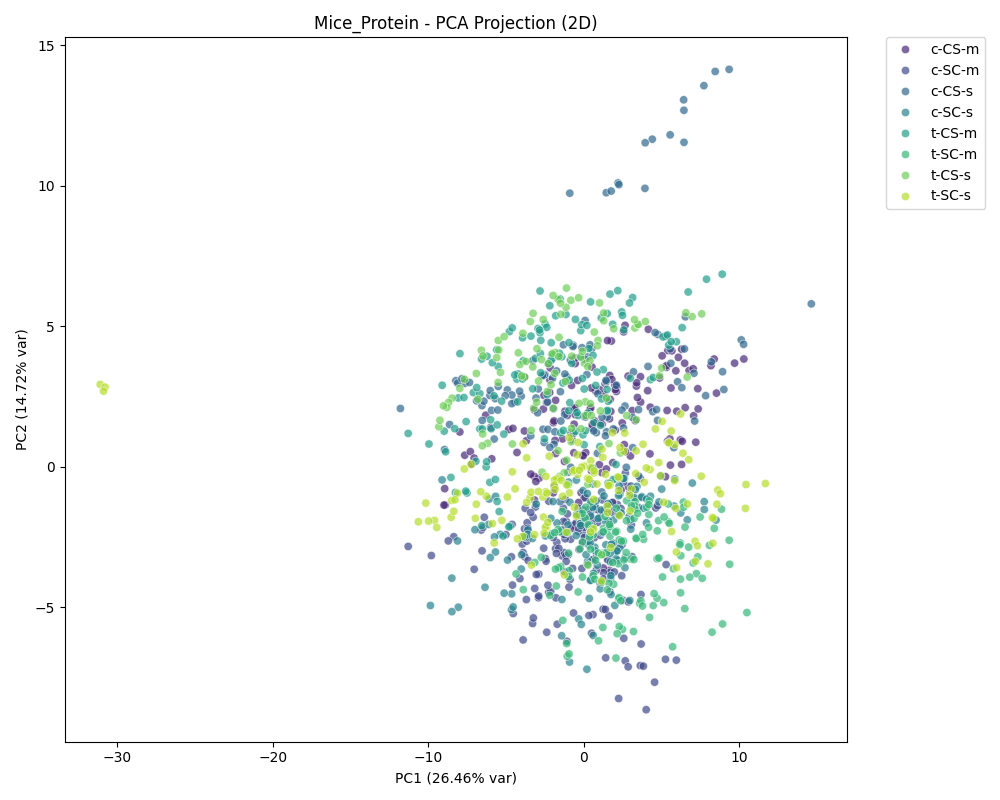
\includegraphics[width=\linewidth]{Mice_Protein_pca.png}
        \caption{PCA Projection (Mice Protein)}
        \label{fig:mice_pca}
    \end{minipage}
    \hfill
    \begin{minipage}{0.48\textwidth}
        \centering
        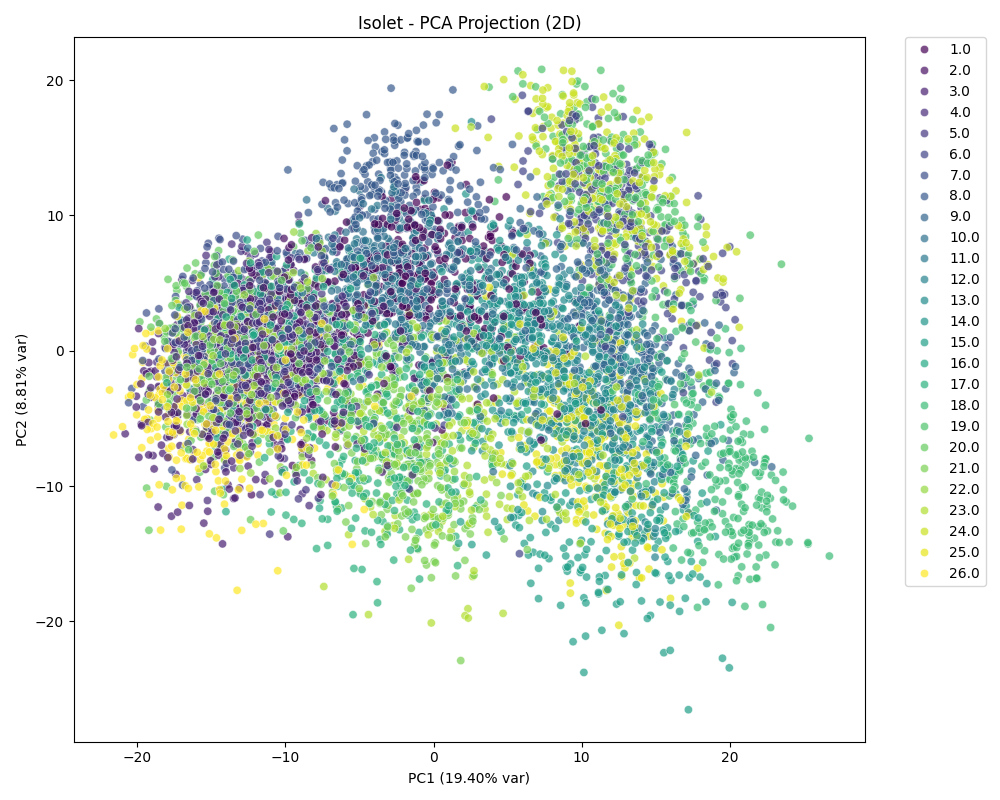
\includegraphics[width=\linewidth]{Isolet_pca.png}
        \caption{PCA Projection (Isolet)}
        \label{fig:isolet_pca}
    \end{minipage}
\end{figure}

\subsubsection{Divide the original dataset into two subsets (80\% - 20\%)}
To strictly adhere to the hold-out validation protocol, we partitioned the datasets into training and testing subsets using the \texttt{train\_test\_split} function from \texttt{sklearn.model\_selection}. We used a fixed \texttt{random\_state=42} to ensure reproducibility.
\begin{enumerate}
    \item \textbf{Training Set (80\%):} 864 samples for Mice Protein, 6237 samples for Isolet. Used for model fitting.
    \item \textbf{Testing Set (20\%):} 216 samples for Mice Protein, 1560 samples for Isolet. Used exclusively for evaluation.
\end{enumerate}

Missing values in the Mice Protein dataset were handled via simple imputation (filling with 0) to ensure compatibility with the sklearn implementation.

\subsection{Build a DT for the training subset}

\subsubsection{Theoretical Background and Algorithm Description}
A Decision Tree is a hierarchical model that partitions the feature space into rectangular regions. The tree structure consists of:
\begin{itemize}
    \item \textbf{Root Node:} Represents the entire dataset.
    \item \textbf{Internal Nodes:} Represent decision points based on a specific feature threshold (e.g., $Feature\_X \leq 0.5$).
    \item \textbf{Leaf Nodes:} Represent the final class assignment.
\end{itemize}

The core algorithm (CART) recursively splits the data to maximize the purity of the resulting subsets. The quality of a split is determined by an impurity metric.

\paragraph{Gini Impurity.} This measures the probability that a randomly selected element from the set would be incorrectly labeled if it were randomly labeled according to the distribution of labels in the subset.
\begin{equation}
    G(S) = 1 - \sum_{i=1}^{c} p_i^2
\end{equation}
where $S$ is the dataset at the node, $c$ is the number of classes, and $p_i$ is the proportion of samples belonging to class $i$. $G=0$ indicates a perfectly pure node.

\paragraph{Entropy (Information Gain).} Alternatively, Entropy measures the uncertainty in the dataset.
\begin{equation}
    H(S) = - \sum_{i=1}^{c} p_i \log_2 p_i
\end{equation}
The algorithm selects the split that maximizes the \textbf{Information Gain}, which is the reduction in Entropy after the split.

\subsubsection{Implementation Details}
We utilized the \texttt{DecisionTreeClassifier} from the \texttt{sklearn.tree} package. The model was initialized with default parameters (Gini criterion) and trained on the 80\% subset. To visualize the decision logic, we generated pruned trees (Depth=3) as shown in Figures \ref{fig:mice_dt_struct} and \ref{fig:isolet_dt_struct}. This visualization helps in interpreting which features are most discriminative at the top levels of the hierarchy.

\begin{figure}[H]
    \centering
    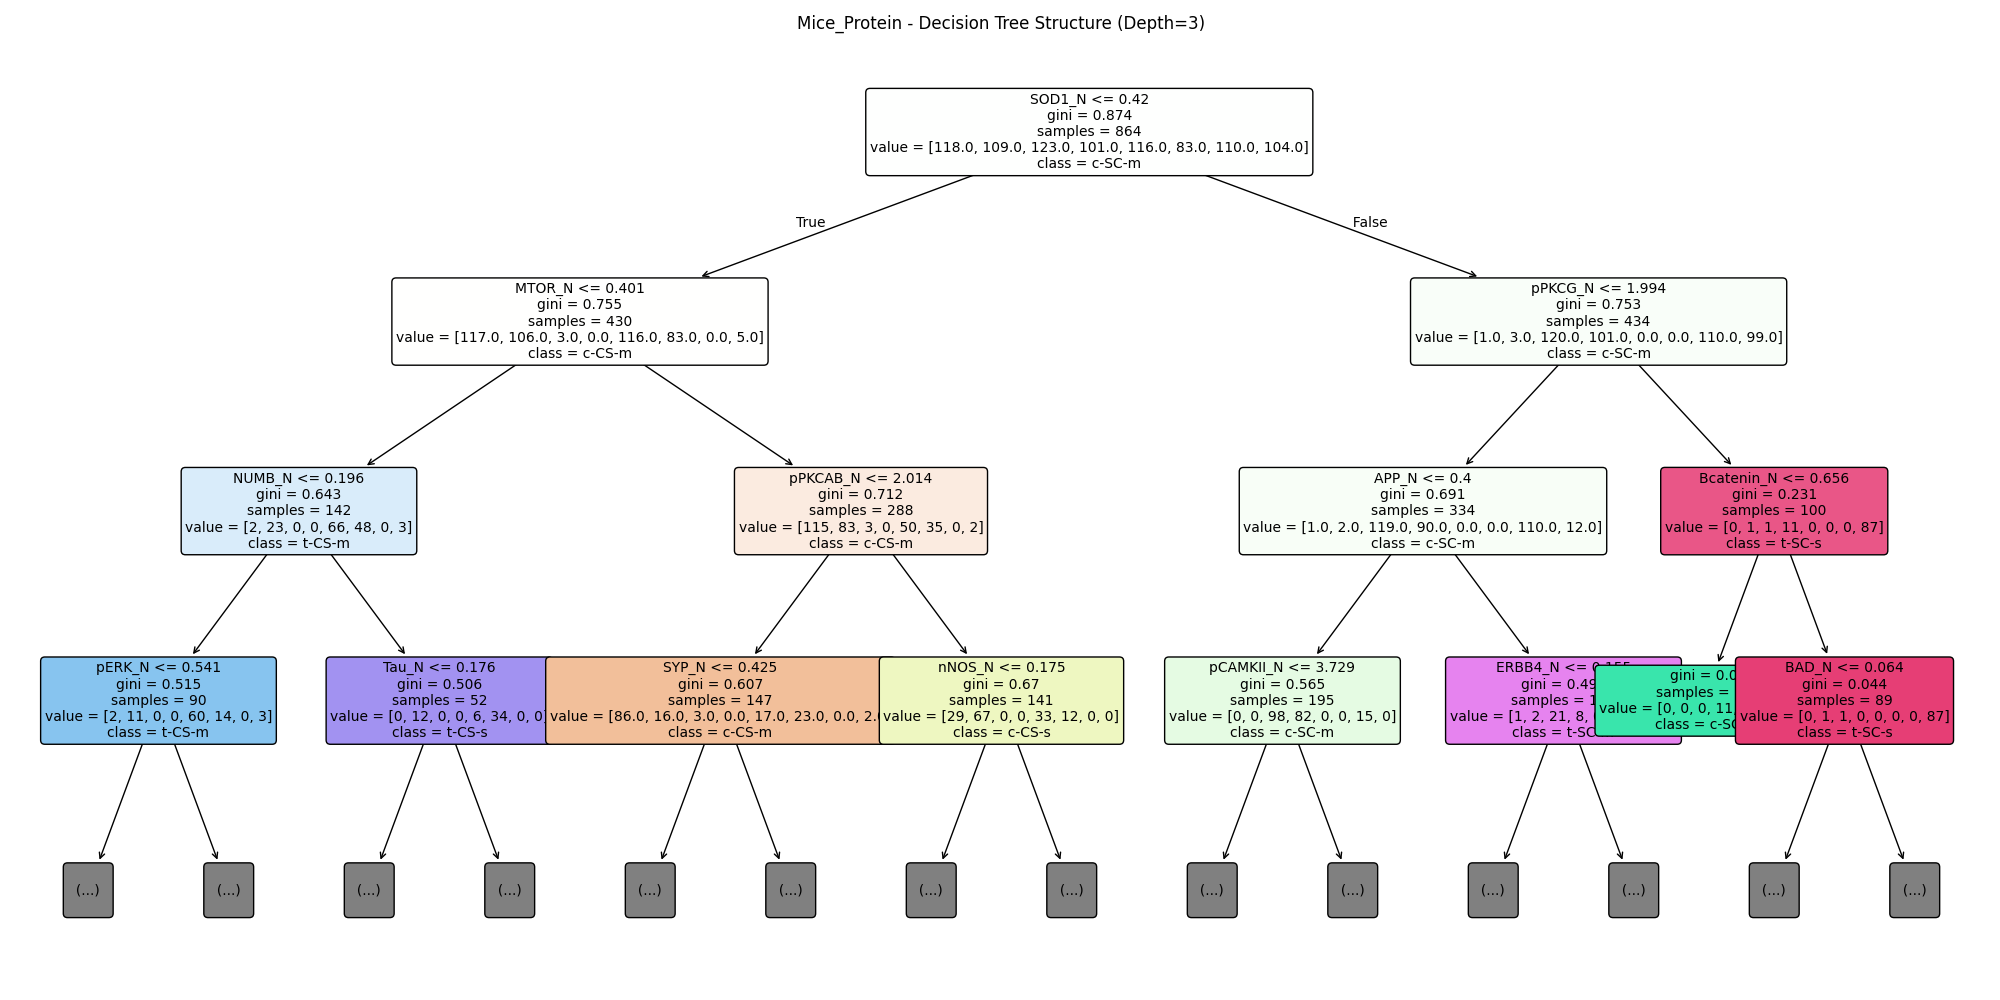
\includegraphics[width=0.9\textwidth]{Mice_Protein_dt_struct.png}
    \caption{Structure of the Decision Tree (Depth=3) for Mice Protein.}
    \label{fig:mice_dt_struct}
\end{figure}

\begin{figure}[H]
    \centering
    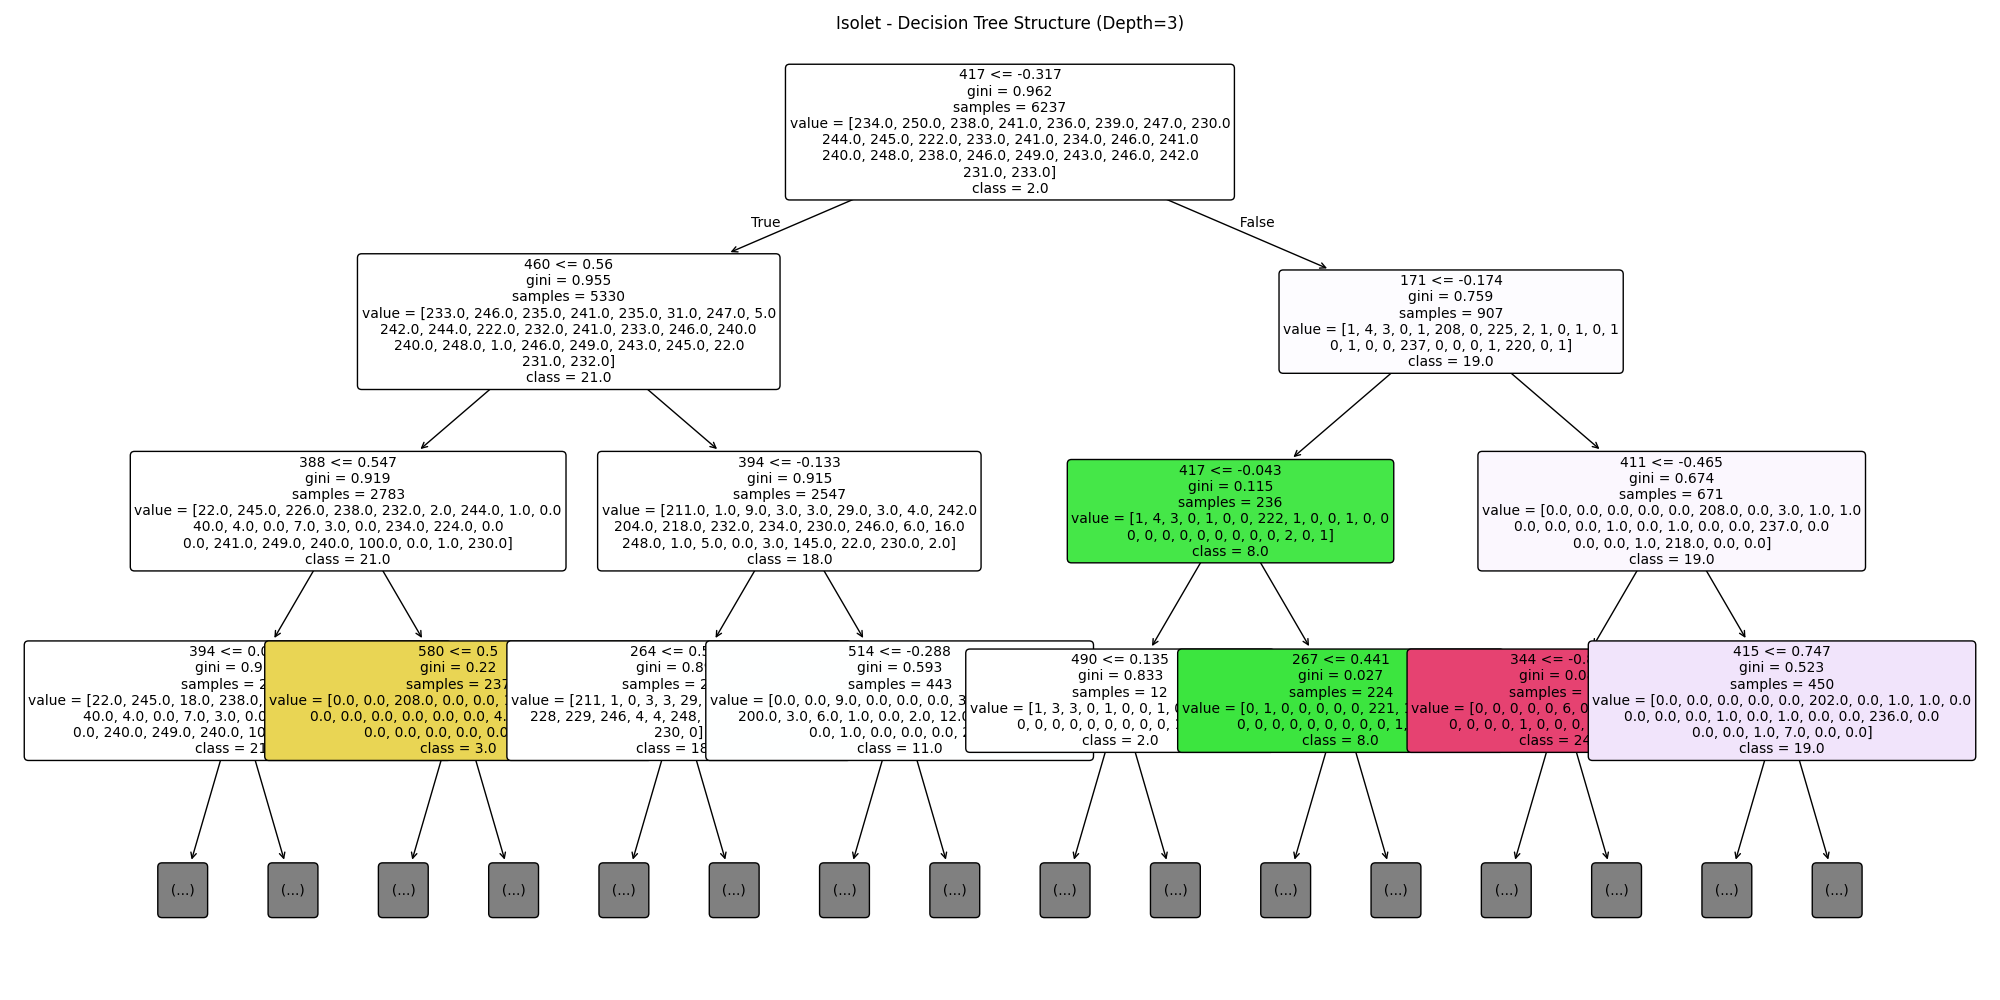
\includegraphics[width=0.9\textwidth]{Isolet_dt_struct.png}
    \caption{Structure of the Decision Tree (Depth=3) for Isolet.}
    \label{fig:isolet_dt_struct}
\end{figure}

\subsection{Calculate the error of classification}

\subsubsection{Performance Metrics}
To provide a comprehensive evaluation, we calculated four key metrics.

\paragraph{Accuracy.} The proportion of correctly classified instances.
\begin{equation}
    \text{Accuracy} = \frac{\text{TP} + \text{TN}}{\text{TP} + \text{TN} + \text{FP} + \text{FN}}
\end{equation}

\paragraph{Precision.} The ratio of correctly predicted positive observations to the total predicted positive observations.
\begin{equation}
    \text{Precision} = \frac{\text{TP}}{\text{TP} + \text{FP}}
\end{equation}

\paragraph{Recall (Sensitivity).} The ratio of correctly predicted positive observations to the all observations in actual class.
\begin{equation}
    \text{Recall} = \frac{\text{TP}}{\text{TP} + \text{FN}}
\end{equation}

\paragraph{F1-score.} The harmonic mean of Precision and Recall.
\begin{equation}
    \text{F1} = 2 \times \frac{\text{Precision} \times \text{Recall}}{\text{Precision} + \text{Recall}}
\end{equation}

For multi-class problems, Precision, Recall, and F1 are calculated as the weighted average across all classes.

\subsubsection{Experimental Results}
The performance of the Decision Tree on the test set is summarized in Table \ref{tab:dt_results}.

\begin{table}[H]
\centering
\begin{tabular}{lccccc}
\toprule
\textbf{Dataset} & \textbf{Accuracy} & \textbf{Error} & \textbf{Precision} & \textbf{Recall} & \textbf{F1-score} \\
\midrule
Mice Protein & 89.81\% & 10.19\% & 0.9017 & 0.8981 & 0.8979 \\
ISOLET & 81.60\% & 18.40\% & 0.8180 & 0.8160 & 0.8157 \\
\bottomrule
\end{tabular}
\caption{Decision Tree Classification Results.}
\label{tab:dt_results}
\end{table}

\paragraph{Analysis.}
For the \textbf{Mice Protein} dataset, the model achieved nearly 90\% accuracy. The confusion matrix (Figure \ref{fig:mice_dt_cm}) shows a strong diagonal, but misclassifications occur between biologically similar classes.
For \textbf{ISOLET}, the accuracy drops to 81.6\%. The high dimensionality (617 features) and the complexity of speech signals likely cause the single decision tree to overfit certain noise patterns in the training data, leading to poorer generalization errors (18.4\%) on the test set. This highlights the limitation of single estimators.

\begin{figure}[H]
    \centering
    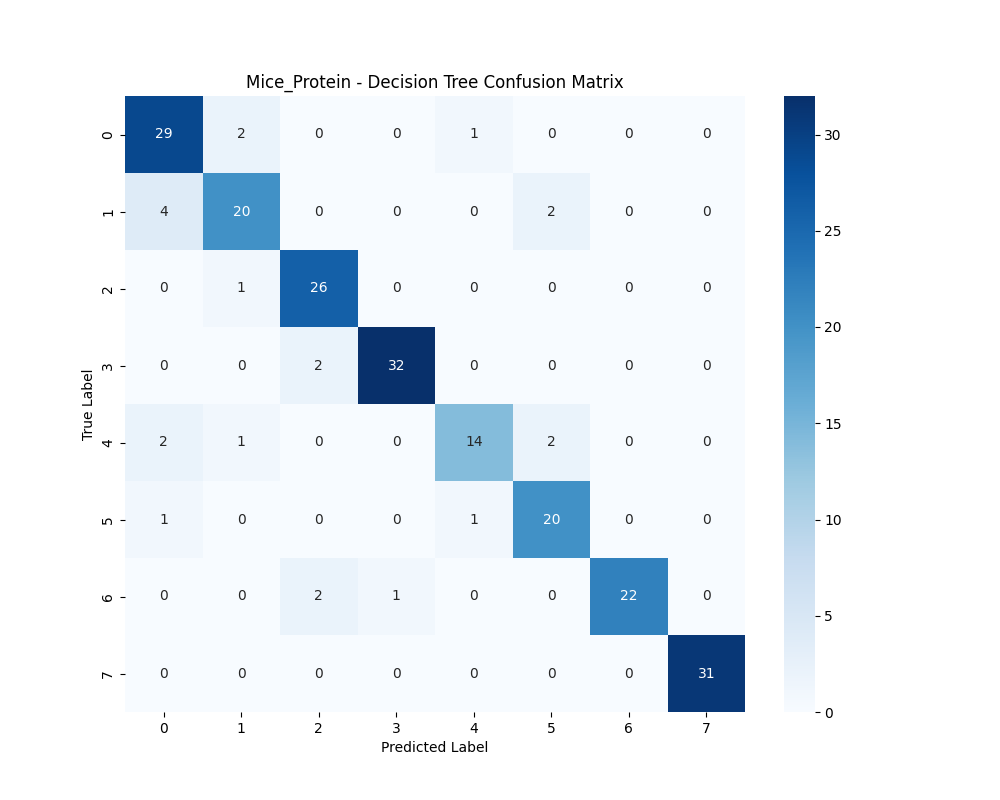
\includegraphics[width=0.6\textwidth]{Mice_Protein_dt_cm.png}
    \caption{Confusion Matrix (DT) - Mice Protein}
    \label{fig:mice_dt_cm}
\end{figure}

\begin{figure}[H]
    \centering
    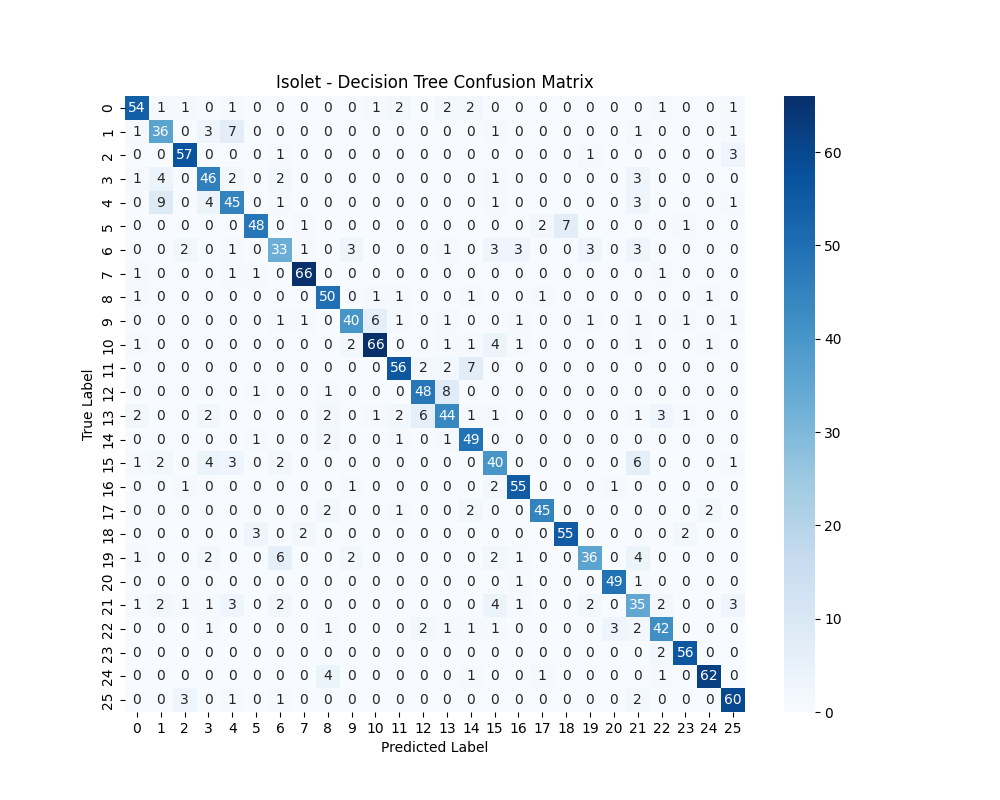
\includegraphics[width=0.7\textwidth]{Isolet_dt_cm.png}
    \caption{Confusion Matrix (DT) - Isolet}
    \label{fig:isolet_dt_cm}
\end{figure}

\section{Random Forest - RF}

\subsection{Analyze and pre-process the data}
The data analysis and pre-processing steps (including PCA, class distribution analysis, and handling missing values) are identical to those described in Section 1.2, ensuring a fair comparison between the two models on the exact same data splits.

\subsection{Create K = 100 training set and build 1 testing set}

\subsubsection{Theoretical Background: Ensemble Learning}
Random Forest is an ensemble learning method that improves upon valid Decision Trees by aggregating the predictions of multiple individual trees ($K$ trees). It employs two main techniques to reduce variance:

\paragraph{1. Bagging (Bootstrap Aggregating).} 
For each tree $T_k$ (where $k=1 \dots K$), we create a new training set $D_k$ by sampling $N$ examples from the original dataset $D$ uniformly and \textbf{with replacement}. This means some samples may appear multiple times in $D_k$, while others are omitted (On average, $\approx 63.2\%$ of unique samples are included).

\paragraph{2. Feature Randomness.}
When splitting a node during tree construction, instead of searching for the best split among all $M$ features, Random Forest searches for the best split among a random subset of $m$ features (typically $m = \sqrt{M}$). This decorrelates the trees, ensuring that they do not all rely on the same dominant features.

\subsubsection{Validation of K=100 (Convergence Analysis)}
We constructed $K=100$ training sets using the bagging technique. To verify that 100 trees are sufficient, we analyzed the \textbf{OOB (Out-of-Bag) / Test Error convergence}. 
Figures \ref{fig:mice_rf_conv} and \ref{fig:isolet_rf_conv} plot the classification error against the number of trees. The error rate drops sharply initially and stabilizes around 40-50 trees. Using $K=100$ ensures we are well into the stable region, minimizing variance.

\begin{figure}[H]
    \centering
    \begin{minipage}{0.48\textwidth}
        \centering
        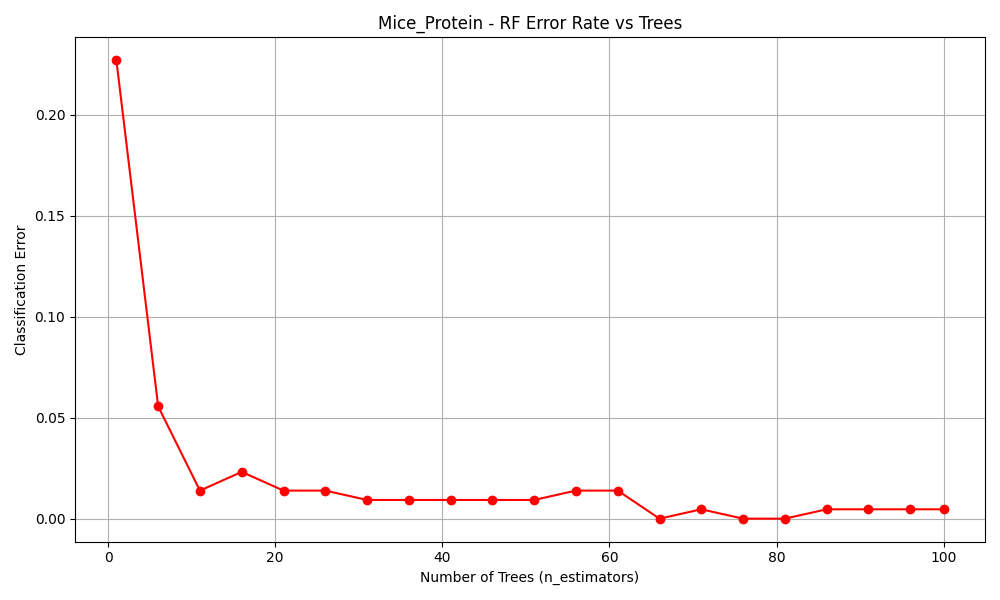
\includegraphics[width=\linewidth]{Mice_Protein_rf_conv.png}
        \caption{Error vs Trees (Mice)}
        \label{fig:mice_rf_conv}
    \end{minipage}
    \hfill
    \begin{minipage}{0.48\textwidth}
        \centering
        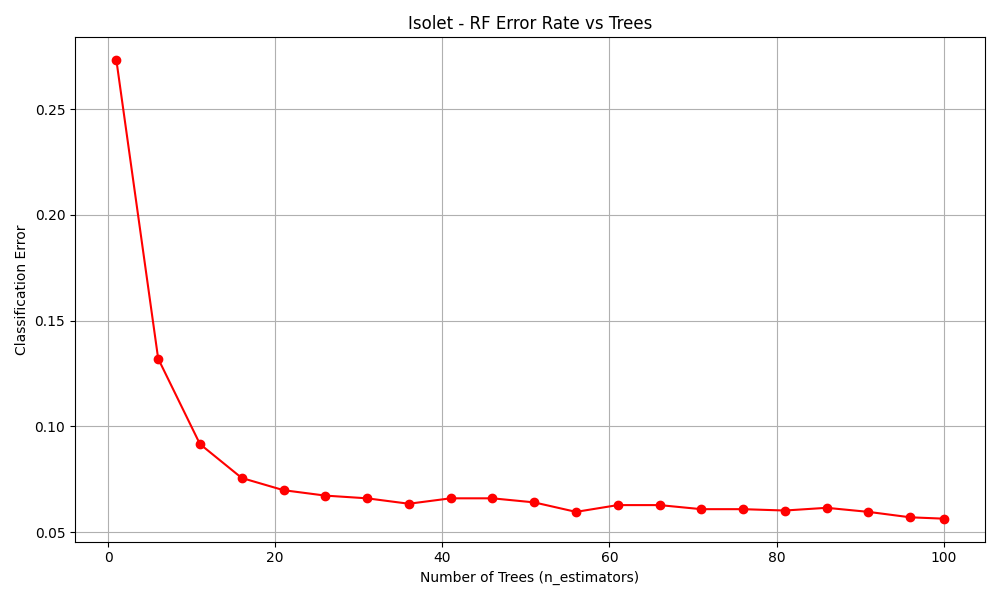
\includegraphics[width=\linewidth]{Isolet_rf_conv.png}
        \caption{Error vs Trees (Isolet)}
        \label{fig:isolet_rf_conv}
    \end{minipage}
\end{figure}

\subsection{Build an RF and calculate the error of classification}

We trained the Random Forest classifier ($K=100, \text{random\_state}=42$) on the training subsets and classified the data from the testing subsets using majority voting.

\begin{table}[H]
\centering
\begin{tabular}{lccccc}
\toprule
\textbf{Dataset} & \textbf{Accuracy} & \textbf{Error} & \textbf{Precision} & \textbf{Recall} & \textbf{F1-score} \\
\midrule
Mice Protein & 99.54\% & 0.46\% & 0.9955 & 0.9954 & 0.9954 \\
ISOLET & 94.36\% & 5.64\% & 0.9451 & 0.9436 & 0.9438 \\
\bottomrule
\end{tabular}
\caption{Random Forest Classification Results (K=100).}
\label{tab:rf_results}
\end{table}

\subsection{Compare the results of RF and DT}

\subsubsection{Quantitative Comparison}
Table \ref{tab:comparison} provides a direct comparison of the two methods.

\begin{table}[H]
\centering
\begin{tabular}{lcccc}
\toprule
\textbf{Dataset} & \textbf{DT Accuracy} & \textbf{RF Accuracy} & \textbf{Improvement} & \textbf{Error Reduction} \\
\midrule
Mice Protein & 89.81\% & \textbf{99.54\%} & +9.73\% & \textbf{95.5\%} \\
ISOLET & 81.60\% & \textbf{94.36\%} & +12.76\% & \textbf{69.3\%} \\
\bottomrule
\end{tabular}
\caption{Comparison: Random Forest vs. Decision Tree.}
\label{tab:comparison}
\end{table}

\subsubsection{Qualitative Analysis and Comment}

\paragraph{Performance Improvement.} Random Forest drastically outperforms the single Decision Tree. For the Mice Protein dataset, the error was virtually eliminated (reduced by 95.5\%). For Isolet, accurate classification increased by nearly 13 percentage points.

\paragraph{Bias-Variance Tradeoff.} The primary reason for this improvement is the reduction of \textbf{Variance}. Single Decision Trees are prone to overfitting—they grow deep and memorize noise in the training data. By averaging 100 trees trained on bootstrapped data, Random Forest smooths out these idiosyncrasies. The decision boundary becomes more robust and generalizable.

\paragraph{Feature Importance.} Random Forest also allows us to inspect which features drive the decisions. Figures \ref{fig:mice_rf_feat} and \ref{fig:isolet_rf_feat} show the top 20 most important features. For Mice Protein, certain key proteins dominate the classification, aligning with biological expectations. For Isolet, specific spectral frequencies are more critical for distinguishing phonemes.

\begin{figure}[H]
    \centering
    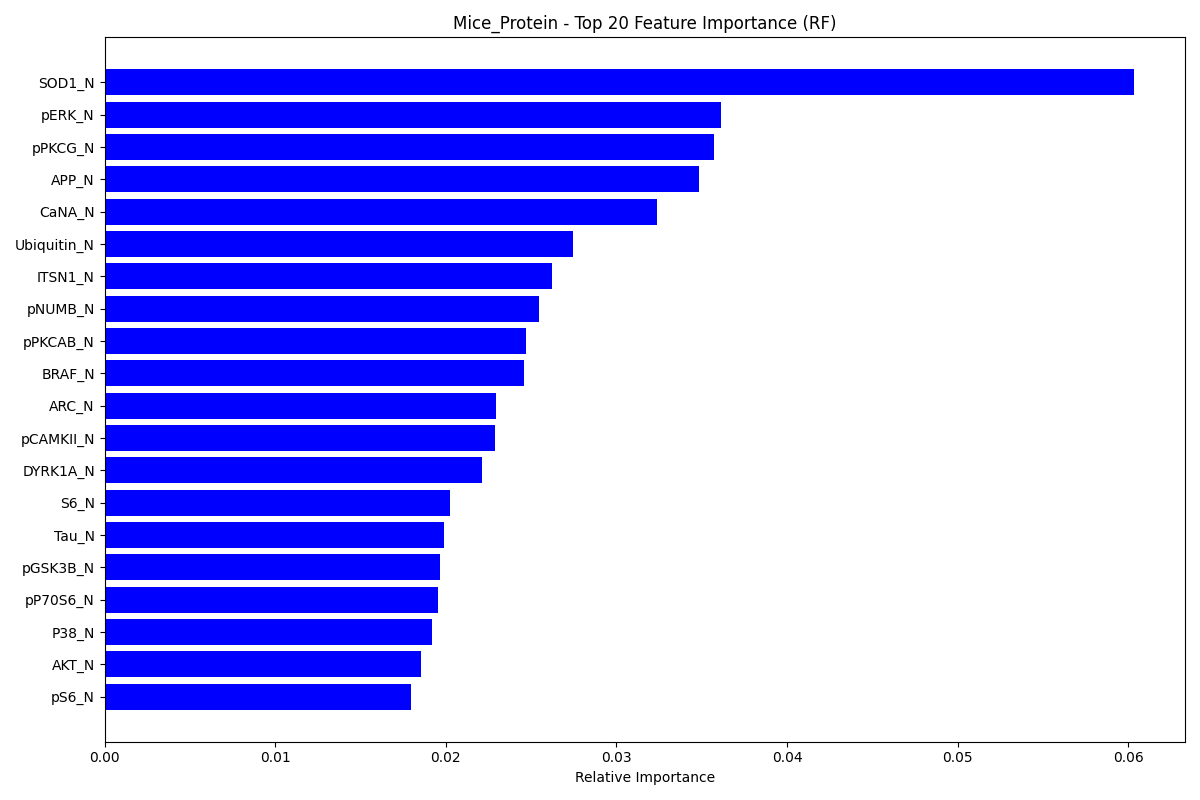
\includegraphics[width=0.8\textwidth]{Mice_Protein_rf_features.png}
    \caption{Top 20 Feature Importance (Mice Protein)}
    \label{fig:mice_rf_feat}
\end{figure}

\begin{figure}[H]
    \centering
    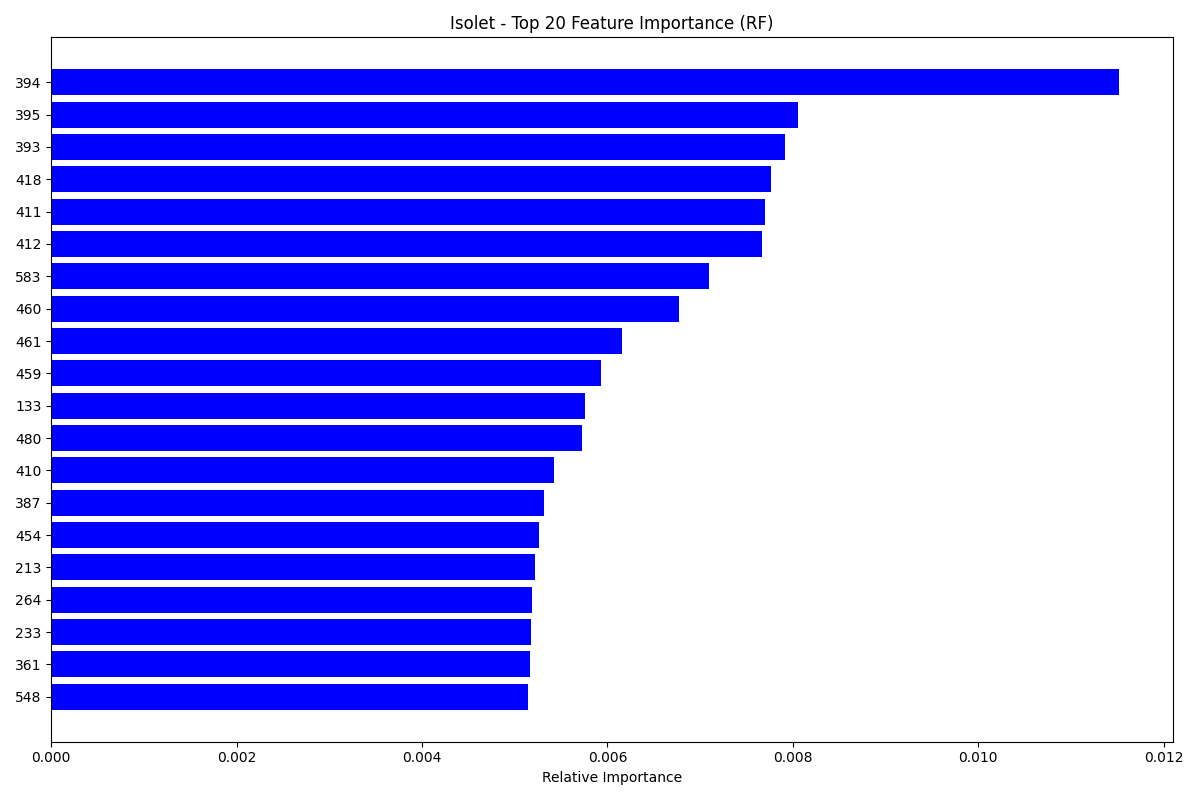
\includegraphics[width=0.8\textwidth]{Isolet_rf_features.png}
    \caption{Top 20 Feature Importance (Isolet)}
    \label{fig:isolet_rf_feat}
\end{figure}

\end{document}
